\documentclass[a4paper,12pt,final]{memoir}

\usepackage{src/components/common}


%%%%%%%%%%%%%%%%%%%%%%%%%%%%%%%%%%%%%
% Create column layout
%%%%%%%%%%%%%%%%%%%%%%%%%%%%%%%%%%%%%
% define length commands
\setlength{\vcolumnsep}{\baselineskip}
\setlength{\columnsep}{\vcolumnsep}

% left frame
\newflowframe{0.26\textwidth}{\textheight}{0pt}{0pt}[left]
	\newlength{\LeftMainSep}
	\setlength{\LeftMainSep}{0.26\textwidth}
	\addtolength{\LeftMainSep}{1\columnsep}
 
% small static frame for the vertical line
\newstaticframe{1.5pt}{\textheight}{\LeftMainSep}{0pt}
 
% content of the static frame
\begin{staticcontents}{1}
\hfill
\tikz{%
	%\draw[loosely dotted,color=RoyalBlue,line width=1.5pt,yshift=0]
	\draw[color=RoyalBlue,line width=\lineTickness,yshift=0]
	(0,0) -- (0,\textheight);}%
\hfill\mbox{}
\end{staticcontents}
 
% right frame
\addtolength{\LeftMainSep}{1.5pt}
\addtolength{\LeftMainSep}{1\columnsep}
\newflowframe{0.64\textwidth}{\textheight}{\LeftMainSep}{0pt}[main01]



%%%%%%%%%%%%%%%%%%%%%%%%%%%%%%%%%%%%%
% Begin document
%%%%%%%%%%%%%%%%%%%%%%%%%%%%%%%%%%%%%
\begin{document}

% Left frame
%%%%%%%%%%%%%%%%%%%%
%
% Picture
\begin{figure}
	\hfill
	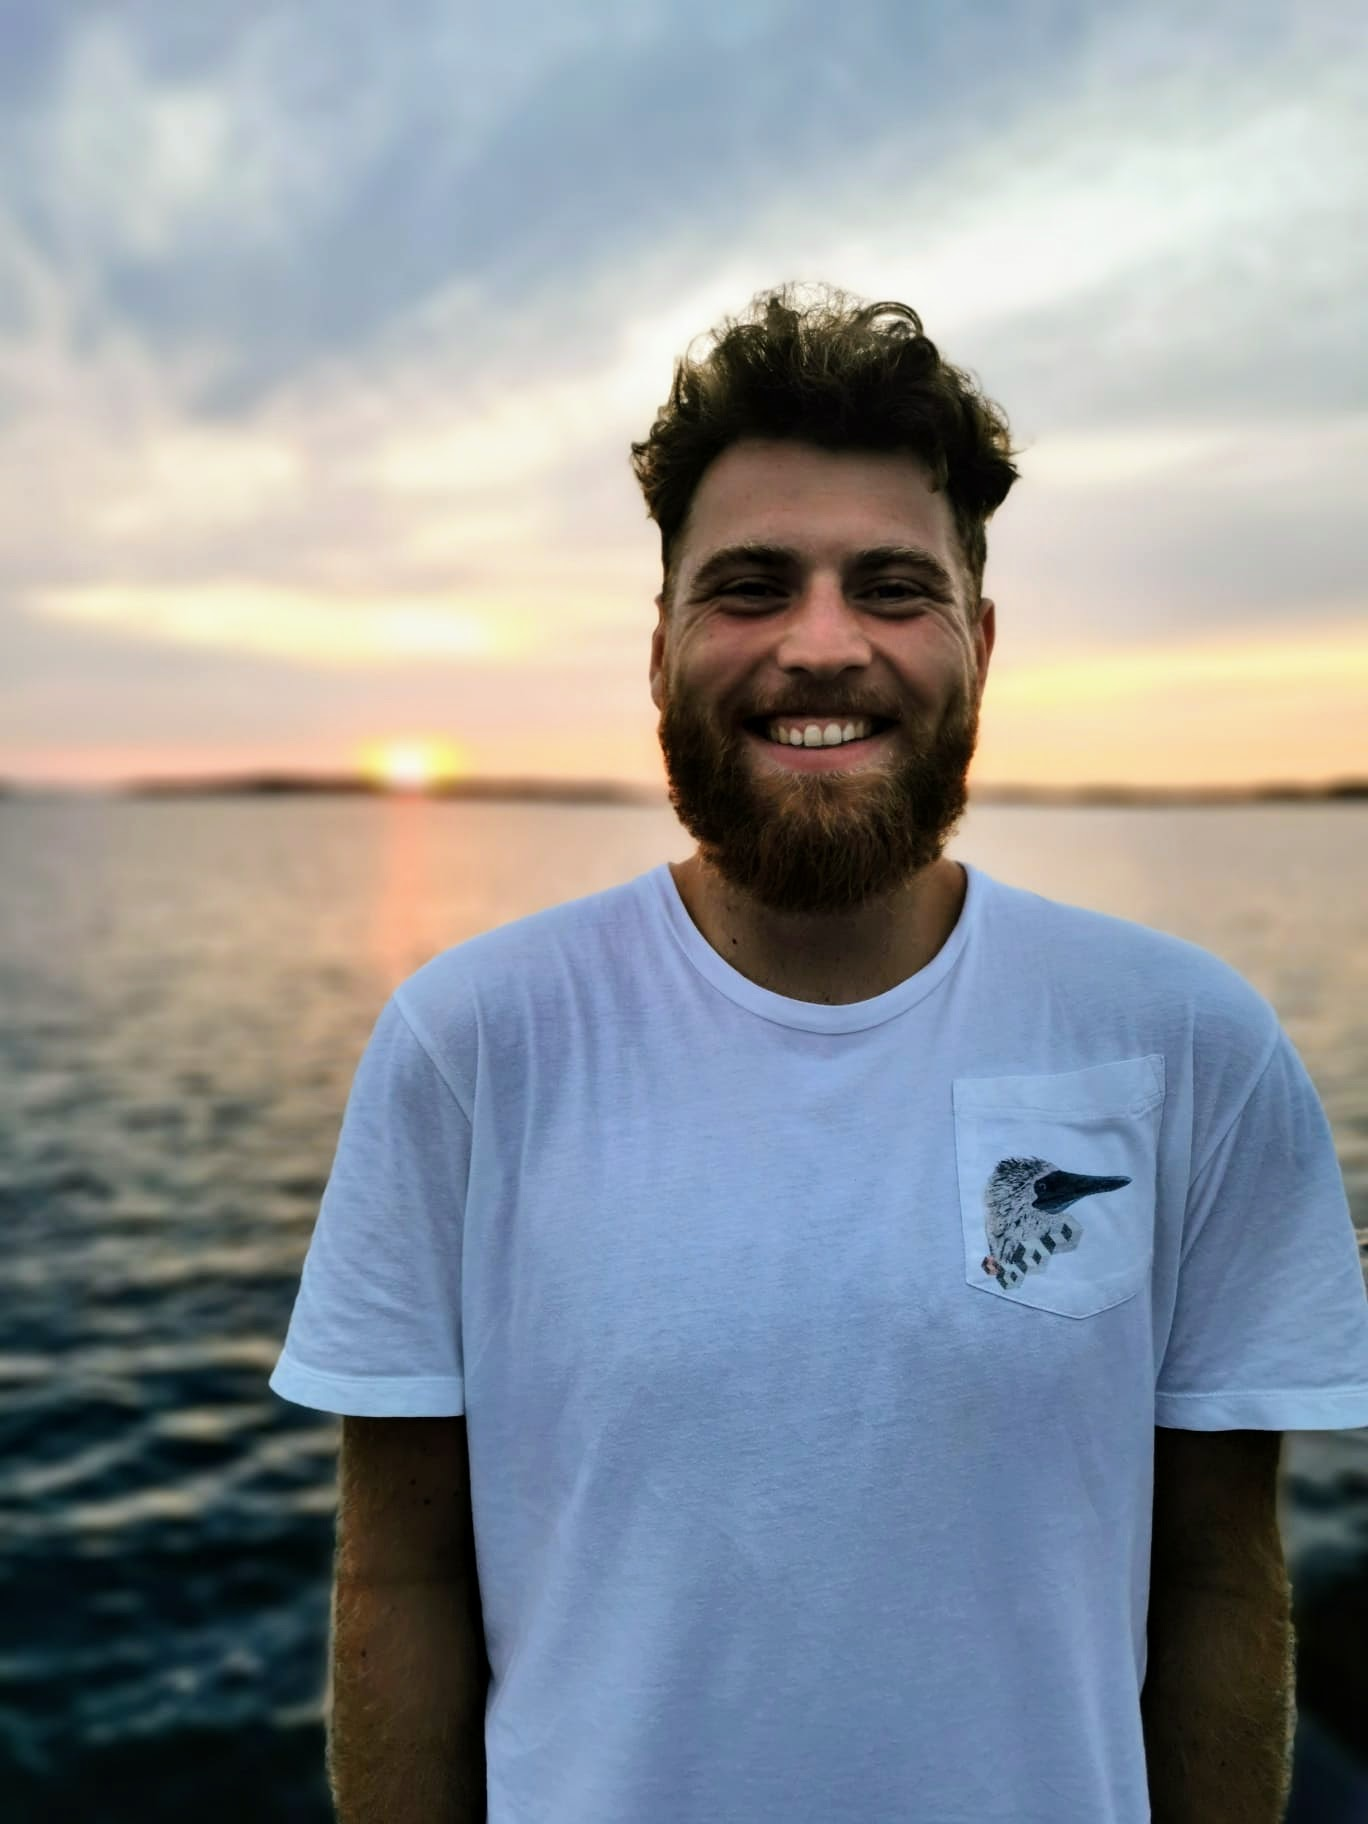
\includegraphics[width=1\columnwidth]{img/profile_pic.jpg}
	\vspace{-3.5cm}
\end{figure}

\begin{flushright}\small
	Wouter Dankers \\
	G\"oteborg, Sweden \\
	+46 (0)720 130 370 \\
	\url{wouter.dankers@skynet.be}  \\
	\url{dankersw.github.io} \\
	\url{github.com/DankersW} \\
	\Sep
	
	% Languages
	{\Large\textbf{Languages}}
	\skills{{Dutch/5}} \\
    \skills{{English/5}} \\
    \skills{{French/1}} \\
    \skills{{Swedish/2.5}} \\
	\Sep
	\Sep
	
	% Interests
    {\Large\textbf{Interests}}\\
	\SmallSep
    \framebox(65,15){Outdoor life} \framebox(57,15){Ice-hockey} \framebox(75,15){Skateboarding} \framebox(40,15){Surfing} \framebox(40,15){Cycling} \framebox(35,15){Skiing} \framebox(25,15){IoT} \framebox(60,15){Automation} \framebox(35,15){Nature} \framebox(45,15){Robotics} \framebox(60,15){Smart-cities} \\
    \Sep

    
\end{flushright}\normalsize
\framebreak

% Right frame
%%%%%%%%%%%%%%%%%%%%
\Huge\bfseries {\color{RoyalBlue} Wouter Dankers} \\
\Large\bfseries  System Engineer \\

\normalsize\normalfont

% About me
\begin{AboutMe}
I am an experienced and versatile software engineer that takes great pride in writing well functioning and clean code that scales and ages well. I am organized, open minded, and efficient, with attention to detail and I have excellent people skills.

\end{AboutMe}

% Experience
\CVSection{Experience}
\CVItem{Apr 2021 - present, Vinnter AB} \hfill G\"oteborg, Sweden \\
\emph{Embedded Software Engineer}
\SmallSep

\CVItem{Jun 2018 - Apr 2021, Volvo Group} \hfill G\"oteborg, Sweden \\
\emph{System Engineer}
\SmallSep

\CVItem{Feb 2016 - Jun 2016, Memory x design} \hfill Beijing, China \\
\emph{Internship}
\Sep

\CVSection{Tech stack}
\begin{multicols}{3}
\begin{compactitem}[\color{RoyalBlue}$\circ$]
	\item Go
	\item C/C++ 
	\item Python
	\item RTOS (Zephyr) 
	\item Bash
	\item C-ITS
	\item Networking
	\item Git
	\item Embedded-Systems
	\item Cloud (GCP, AWS, Azure)
	\item Agile 
	\item Docker
	\item Automation
	\item IoT
	\item Linux
	\item Micro-services
	\item Wireless communication
	\item BLE, Thread, WiFi, Mesh
	\item CI/CD
	\item Databases
\end{compactitem}
\end{multicols}
\Sep

% Education
\CVSection{Education}
\CVItem{2016 - 2018, Halmstad University} \hfill Halmstad, Sweden \\
MSc. Embedded and Intelligent systems
\SmallSep

\CVItem{2013 - 2016, Thomas More Hogeschool} \hfill Geel, Belgium \\
BSc. ICT and Telecommunication
\Sep

% Publications
\CVSection{Publications}
\CVItem{Characterizing Packet Losses in Vehicular Networks} \hfill 2019 \\
Published in \emph{IEEE Transactions on Vehicular Technology}. The Paper is based on the results of my master thesis.
\SmallSep

\CVItem{Modeling Packet Losses in Communication Networks} \hfill 2018 \\
Published in \emph{IEEE International Symposium on Information Theory (ISIT)}.
\Sep

%%%%%%%%%%%%%%%%%%%%%%%%%%%%%%%%%%%%%
% End document
%%%%%%%%%%%%%%%%%%%%%%%%%%%%%%%%%%%%%
\end{document}